\subsection{Simulated Annealing}

Simulated annealing is a stochastic algorithm that attempts to find the global optimum of an objective function $f(x)$. The method is inspired by statistical physics, in particular the Boltzmann distribution that specifies the probability of being in a particular state $x$:
\begin{equation}
    p(x) \propto \exp\{-f(x)/T\}
\end{equation}
where $f(x)$ is the energy of the system and $T$ is the temperature. As the temperature approaches zero, the system spends more and more time in its minimum energy (most probable) state. As the temperature decreases, the largest peaks become larger and the smallest peaks dissappear. By cooling slowly enough, it is possible to track the largest peak and therefore find the global optimum.\\

Simulated annealing is closely related to the Metropolis-Hastings algorithm for generating samples from a probability distribution. At each step of the algorithm, we sample a new state according to a proposal distribution $x^{\prime} \sim q(\dot|x_k)$, such as a random walk proposal:
\begin{equation}
    x^{\prime} = x_k + \epsilon_k, ~~~ \mathrm{where}~ \epsilon_k \sim N(0,\Sigma)
\end{equation}
Having proposed a new state, we compute $\alpha$ as in Algorithm \ref{alg:sim_annealing}.
\begin{algorithm}
\caption{Simulated Annealing}
\label{alg:sim_annealing}
\begin{algorithmic}[1]
\STATE $\alpha = \exp\{(f(x)-f(x^{\prime}))/T\}$
\STATE $r = \min(1,\alpha)$
\STATE $u \sim \mathrm{Unif}(0,1)$
\STATE if $u < r$ 
\STATE ~~~ $x_{k+1} = x^{\prime}$
\STATE else
\STATE ~~~ $x_{k+1} = x_k$
\STATE end if  
\end{algorithmic}
\end{algorithm}
Thus, if a new state has lower energy (higher probability), we will definitely accept it but if it has higher energy (lower probability), we might still accept it depending on the temperature. Therefore, the algorithm allows downhill moves in probability space but less frequently as the temperature drops. In practice it is common to use an exponential cooling schedule: $T_k = T_0 C^{k}$, where $T_0 \sim 1$ is the initial temperature and $C \sim 0.8$ is the cooling rate. Cooling too quickly can result in getting stuck in local optima, while cooling too slowly wastes time. The optimum cooling schedule is difficult to determine.    

\begin{figure}[tbhp]
    \centering
    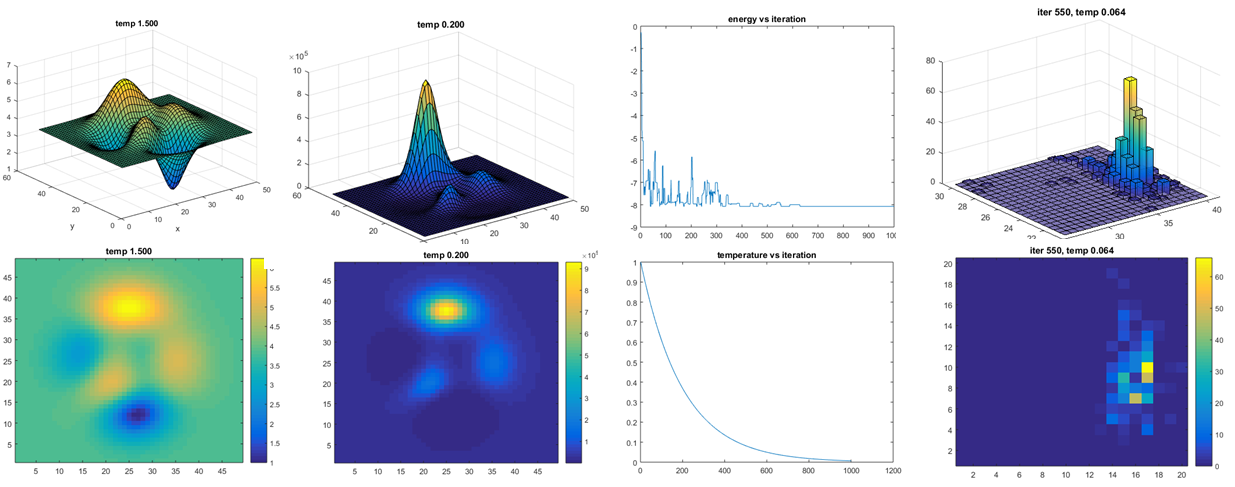
\includegraphics[width=0.9\textwidth, trim={10 10 10 10}]{figures/sim_annealing_merged.png}
    \caption{Simulated Annealing}
    \label{fig:sim_annealing_merged}
\end{figure}

Figure \ref{fig:sim_annealing_merged} shows the objective $f(x)$ at two different temperatures (left). The function appears more peaky when the temperature is lower. We can also see that the method stochastically reduces the energy over time for the given cooling schedule (middle). Finally a histogram of samples shows that most samples are concentrated near the global maximum (right).


\subsection{Bayesian Optimization}

Machine learning algorithms frequenty require careful tuning of hyperparameters. Often exhaustive and computationally expensive methods such as grid search cross validation are used to find model parameters that optimize a suitable performance objective. An alternative to grid search is randomized parameter optimization that samples parameter settings from a distribution over possible parameter values. This has two main benefits over the exhaustive search: the number of iterations can be chosen independent of the number of parameters and adding parameters that do not influence performance does not decrease efficiency. Rather than exploring the parameter space randomly (according to a chosen distribution), it would be great to adapt an active learning approach that selects parameter values in a way that reduces uncertainty and provides a balance between exploration and exploitation. Bayesian optimization provides an automated Bayesian framework by utilizing Gaussian Processes (GPs) to model algorithm's generalization performance \cite{snoek2012}.\\

Bayesian optimization assumes that a suitable performance function was sampled from a Gaussian Process and maintains a posterior distribution for this function as observations are made: $f(x)\sim \mathrm{GP}(m(x),\kappa(x,x^{\prime}))$. To choose which hyperparameters to explore next, one can optimize the Expected Improvement (EI) over the current best result or the Gaussian process Upper Confidence Bound (UCB). EI and UCB have been shown to be efficient in the number of function evaluations required to find the global optimum of multi-modal black-box functions. Bayesian optimization uses all of the information available from previous evaluations of the objective function as opposed to relying on local gradient and Hessian approximations. This results in an automated procedure that can find an optimum of non-convex functions with relatively few evaluations, at the cost of performing more computation to determine the next point to try. This is particularly useful when evaluations are expensive to perform such as in selecting hyperparameters for deep neural networks.\\

To determine what point should be evaluated next, we need to choose and acquisition function which is used to construct a utility function from the GP posterior. In general, the acquisition function depends on previous observations as well as GP hyperparameters that we denote as $a(x;\{x_n,y_n\},\theta)$, then $x_{next} = \arg \max_x a(x)$. Let $\mu(x;\{x_n,y_n\},\theta)$ be the predictive GP mean function, $\sigma^{2}(x;\{x_n,y_n\},\theta)$ be the predictive GP variance function and $\Phi(x)$ be the cumulative distribution function of the standard normal. Then we can define the following acquisition functions.\\

\textit{Probability of Improvement}. This strategy maximizes the probability of improving over the best current value. This can be computed as follows:
\begin{equation}
    a_{PI}(x;\{x_n,y_n\},\theta) = \Phi(\gamma(x)), ~~~~ \gamma(x) = \frac{f(x_{best}) - \mu(x; \{x_n,y_n\},\theta)}{\sigma(x;\{x_n,y_n\},\theta)}
\end{equation}

\textit{Expected Improvement}. Alternatively, one could choose to maximize the expected improvement (EI) over the current best. 
\begin{equation}
    a_{EI}(x;\{x_n,y_n\},\theta) = \sigma(x;\{x_n,y_n\},\theta)(\gamma(x)\Phi(\gamma(x))+N(\gamma(x);0,1))
\end{equation}

\textit{Upper Confidence Bound}. UCB is the idea of exploiting upper confidence bounds to construct acquisition functions that minimize regret over the course of their optimization. These acquisition functions have the following form:
\begin{equation}
    a_{UCB}(x;\{x_n,y_n\},\theta) = \mu(x;\{x_n,y_n\},\theta) - \kappa \sigma(x;\{x_n,y_n\},\theta)
\end{equation}
where $\kappa$ is a tunable acquisition parameter to balance exploration and exploitation. The optima of acquisition functions are located where the uncertainty in GP posterior is large (exploration) and/or where the GP prediction is high (exploitation). Since acquisition functions have analytical forms that are simple to evaluate, they are easier to optimize then the original objective function.\\

An important practical consideration for Bayesian optimization is an appropriate choice of GP kernel and its associated hyperparameters. Squared exponential kernel is often a default choice for Gaussian process regression. However, sample functions with this kernel are too smooth for practical optimization problems. Instead the following ARD Matern $5/2$ kernel is proposed:
\begin{eqnarray}
    K_{M52}(x,x^{\prime}) &=& \theta_0\bigg(1+\sqrt{5r^2(x,x^{\prime})}+\frac{5}{3}r^2(x,x^{\prime}) \bigg)\exp \{-\sqrt{5r^2(x,x^{\prime})}\}\\
    r^2(x,x^{\prime}) &=& \sum_{d=1}^{D}(x_d - x^{\prime}_d)^{2}/\theta_{d}^{2}
\end{eqnarray}
This kernel results in sample functions that are twice-differentiable without requiring the smoothness of the squared exponential kernel. The associated kernel hyperparameters are $D$ length scales $\theta_{1:D}$, the covariance amplitude $\theta_0$, the observation noise $\nu$ and a constant mean $m$. An additional assumption made by GP regression is that the underlying process is stationary, i.e. we can re-write the kernel $k(x,x^{\prime})$ as a function of $x-x^{\prime}$. Intuitively, a function whose length scale does not change throughout the input space will be modelled well by a GP with a stationary kernel.\\ 

Bayesian Optimization algorithm is summarized in Algorithm \ref{alg:bayes_opt}.
\begin{algorithm}
\caption{Bayesian Optimization}
\label{alg:bayes_opt}
\begin{algorithmic}[1]
\STATE \textbf{for} $n=1,2,...$ \textbf{do}
\STATE ~~~ select new $x_{n+1}$ by optimizing acquisition function $\alpha$\\
~~~ ~~~ $x_{n+1} = \arg \max_x \alpha(x;D_n,\theta)$
\STATE ~~~ query objective function to obtain $y_{n+1} = f(x_{n+1})$
\STATE ~~~ augment data $D_{n+1} = \{D_n,(x_{n+1},y_{n+1})\}$
\STATE ~~~ update GP posterior and acquisition function 
\STATE \textbf{end for}  
\end{algorithmic}
\end{algorithm}


\begin{figure}[tbhp]
    \centering
    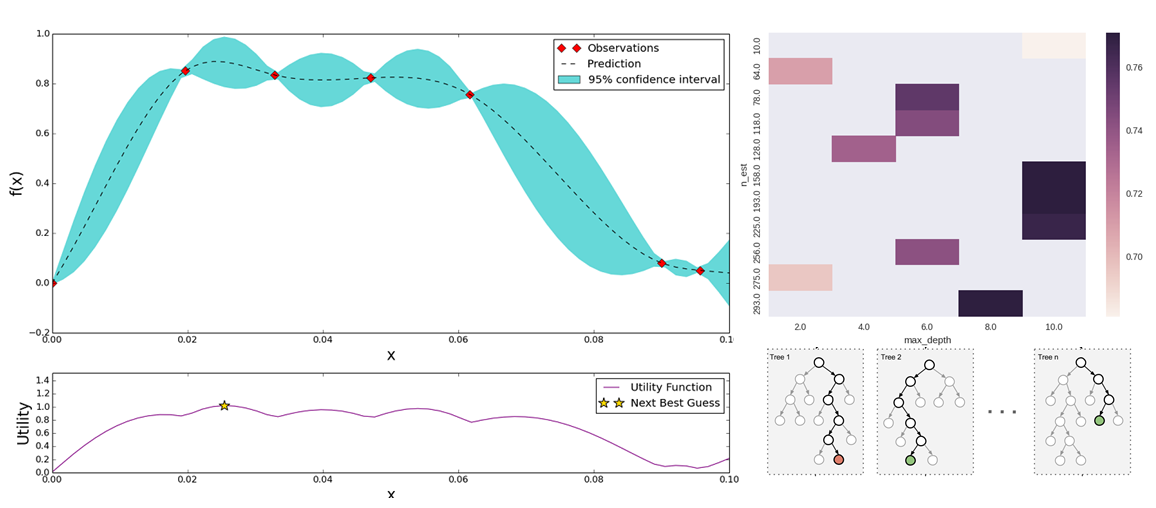
\includegraphics[width=0.95\textwidth, trim={10 10 10 10}]{figures/bayes_opt.png}
    \caption{Bayesian Optimization of SVM and Random Forest parameters}
    \label{fig:bayes_opt}
\end{figure}

Figure \ref{fig:bayes_opt} shows Baeysian optimization applied to SVM and Random Forest. F1 score was used as performance objective function for a classification task. The figure on the left shows Bayesian optimization of F1 score as a function of the gamma parameter of the SVM RBF kernel: $K(x,x^{\prime}) = \exp\{-\gamma ||x-x^{\prime}||^{2}\}$. We can see that after only 7 iterations we have discovered the gamma parameter that gives the maximum F1 score. The peak of EI utility function at the bottom tells us which experiment to perform next. The figure on the right shows Bayesian optimization of F1 score as a function of maximum depth and the number of estimators of a Random Forest classifier. From the heatmap, we can tell that the maximum F1 score is achieved for $158$ estimators with depth equal to $10$.    


\subsection{Active Learning}

The key idea behind active learning is that a machine learning algorithm can achieve greater accuracy with fewer training labels if it is allowed to choose the data from which it learns. Active learning is well motivated in many modern machine learning problems where unlabeled data may be abundant but labels are expensive to obtain. Active learning is sometimes called query learning or optimal experimental design because an active learner poses queries in the form of unlabelled data instances to be labeled by an oracle. In this way, the active learner seeks to achieve high accuracy using as few labeled instances as possible \cite{Settles2009}.\\

We focus on \textit{pool-based sampling} that assumes that there is a small set of labeled data $L$ and a large pool of unlabelled data $U$. Queries are selectively drawn from the pool according to an informativeness measure. Pool based methods rank the entire collection of unlabelled data to select the best query. Therefore, for very larget data-sets, stream-based sampling maybe more appropriate where the data is scanned sequentially and query decisions are evaluated individually.\\

\begin{figure}[tbhp]
    \centering
    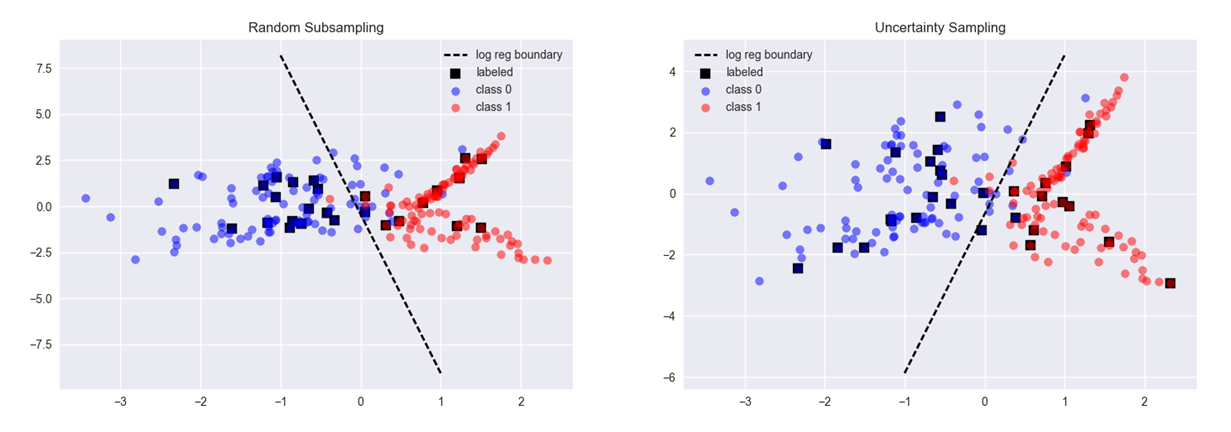
\includegraphics[width=0.95\textwidth, trim={10 10 10 10}]{figures/active_learning_logreg.png}
    \caption{Random Subsampling vs Uncertainty Sampling}
    \label{fig:al_logreg}
\end{figure}

Figure \ref{fig:al_logreg} shows an example of pool-based active learning based on binary classification of a synthetic dataset with two balanced classes using Logistic Regression (LR). On the left, we can see the LR decision boundary as a result of training on a randomly subsampled set of $30$ labels that achieves a classification accuracy of $90\%$ on held out data. On the right, we can see the LR decision boundary as a result of training on $30$ queries selected by uncertainty sampling based on entropy. Uncertainty sampling achieves a higher classification accuracy of $92.5\%$ on the held out set.   


\subsubsection{Query Strategies}

\textit{Uncertainty Sampling.} One of the simplest and most commonly used query framework is uncertainty sampling. In this framework, an active learner queries the label about which it is least certain. For example, in binary logistic regression, uncertainty sampling queries points near the boundary where the probability of being positive is close to $0.5$. For multi-class problems, uncertainty sampling can query points that are least confident:
\begin{equation}
    x_{LC}^{\ast} = \arg \max_x 1 - P_{\theta}(\hat{y}|x)
\end{equation}
where $\hat{y} \in \{1,...,K\}$ is the class label with the highest posterior probability under the model $\theta$. The criterion for the least confident strategy only considers information about the most probable label. We can use max margin sampling to preserve information about the remaining label distribution:
\begin{equation}
    x_{M}^{\ast} = \arg \min_x P_{\theta}(\hat{y}_1|x) - P_{\theta}(\hat{y}_2|x)
\end{equation}
where $\hat{y}_1$ and $\hat{y}_2$ are the first and second most probable class labels under the model, respectively. Intuitively, instances with large margins are easy to classify. Thus, points with small margins are ambiguous and knowing their labels would help the model to more effectively discriminate between them. However, for multi-class problems with very large label sets, the margin strategy still ignores much of the output distribution for the remaining classes. A more general uncertainty sampling strategy is based on entropy:
\begin{equation}
    x_{H}^{\ast} = \arg \max_x -\sum_i P_{\theta}(y_i|x)\log P_{\theta}(y_i|x)
\end{equation}
By learning labels that have highest entropy we can reduce label uncertainty. Uncertainty sampling also works for regression problems, in which case the learner queries the point with highest output variance in its prediction.\\

\textit{Query by Committee.} Another query selection framework is the Query By Committee (QBC) algorithm that involves maintaining a committee $C = \{\theta^{(1)},...,\theta^{(C)}\}$ of models which are all trained on the current labeled set $L$ but represent competing hypotheses. Each committee member is then allowed to vote on the labelings of query candidates and the most informative query is considered to be an instance about which they most disagree. The objective of QBC is to minimize a set of hypotheses that are consistent with the current labeled training data $L$. For measuring the level of disagreement two main approaches have been proposed \cite{Settles2009}: the vote entropy and KL divergence. The vote entropy is defined as follows:
\begin{equation}
    x_{VE}^{\ast} = \arg \max_x - \sum_i \frac{V(y_i)}{C} \log \frac{V(y_i)}{C}
\end{equation}
where $y_i \in \{1,...,K\}$ is the class label, $V(y_i)$ is the number of votes that a label received from the committee members and $C$ is the size of the committee. The KL divergence for QBC voting is defined as follows:
\begin{eqnarray}
    x_{KL}^{\ast} &=& \arg \max_x \frac{1}{C} \sum_{c=1}^{C} KL(P_{\theta^{(c)}}||P_C)\\
    KL(P_{\theta^{(c)}}||P_C) &=& \sum_i P_{\theta^{(c)}}(y_i|x) \log \frac{P_{\theta^{(c)}}(y_i|x)}{P_C(y_i|x)}\\
    P_C(y_i|x) &=& \frac{1}{C}\sum_{c=1}^{C}P_{\theta^{(c)}}(y_i|x)
\end{eqnarray}
where $\theta^{(c)}$ represents a member model of the committee and $P_C(y_i|x)$ is the consensus probability that $y_i$ is the correct label. The KL divergence metric considers the most informative query to be the one with the largest average difference between the label distributions of any one committee member and the consensus distribution.\\

\textit{Variance Reduction}. We can reduce the generalization error by minimizing output variance. Consider a regression problem for which the learning objective is to minimize the mean squared error. Let $\bar{\theta} = E[\hat{\theta}]$ be the expected value of the parameter estimate $\hat{\theta}$ and let $\theta^{\ast}$ be the ground truth, then
\begin{eqnarray}
   \mathrm{MSE} &=& E\bigg[(\hat{\theta} - \theta^{\ast})^{2} \bigg]  = E\bigg[\big[(\hat{\theta} - \bar{\theta})+(\bar{\theta} - \theta^{\ast}) \big]^{2} \bigg] \\
                &=& E\bigg[(\hat{\theta} - \bar{\theta})^{2} \bigg] + 2(\bar{\theta}-\theta^{\ast})E\bigg[\hat{\theta}-\bar{\theta}\bigg] + (\bar{\theta}-\theta^{\ast})^{2} \\
                &=& E\bigg[(\hat{\theta} - \bar{\theta})^{2} \bigg] +  (\bar{\theta}-\theta^{\ast})^{2} \\
                &=& \mathrm{VAR}[\hat{\theta}] + \mathrm{bias}^{2}(\hat{\theta})
\end{eqnarray}
This is called the \textbf{bias-variance tradeoff}. Thus, it is possible to achieve lower MSE with a biased estimator as long as it reduces the variance. A natural question is how low can the variance be? The answer is given by the Cramer-Rao lower bound that provides a lower bound on the variance of any unbiased estimator.
\begin{theorem}
(Cramer-Rao Lower Bound) Assuming $p(x|\theta)$ satisfies the regularity condition, the variance of any unbiased estimator $\hat{\theta}$ satisfies:
\begin{equation}
    \mathrm{VAR}(\hat{\theta}) \geq \frac{1}{-E\big[\frac{\partial^{2} \log p(x|\theta)}{\partial \theta^{2}} \big]} = \frac{1}{I(\theta)}
\end{equation}
where $I(\theta)$ is the Fisher information matrix. 
\end{theorem}
Thus, the Minimum Variance Unbiased (MVU) estimator achieves the minimum variance equal to the inverse of the Fisher information matrix. To minimize variance of parameter estimates, an active learner should select data that maximizes its Fisher information. For multi-variate models with $K$ parameters, Fisher information takes the form of a $K\times K$ matrix:
\begin{equation}
    [I(\theta)]_{ij} = -E \bigg[\frac{\partial^{2}\log p(x|\theta)}{\partial \theta_i \partial \theta_j} \bigg]
\end{equation}
As a result, there are several options for minimizing the inverse information matrix: A-optimality minimizes the trace: $Tr(I^{-1}(\theta))$, D-optimality minimizes the determinant: $|I^{-1}(\theta)|$ and E-optimality minimizes the maximum eigenvalue: $\lambda_{max}[I^{-1}(\theta)]$.\\

However, there are some computational disadvantages to the variance reduction methods. Estimating output variance requires inverting a $K\times K$ matrix for each unlabeled instance, resulting in a time complexity of $\mathcal{O}(UK^{3})$, where $U$ is the size of the query pool. As a result variance reduction methods are empirically slower than simpler query strategies like uncertainty sampling.\\  

Active learning and \textit{semi-supervised learning} both try to make the most of unlabeled data. For example, a basic semi-supervised technique is self-training in which the learner is first trained with a small amount of labeled data and then used to classify the unlabeled data. The most confident unlabeled instances together with their predicted labels are added to the training set and the process repeats.\\ 

\begin{figure}[tbhp]
    \centering
    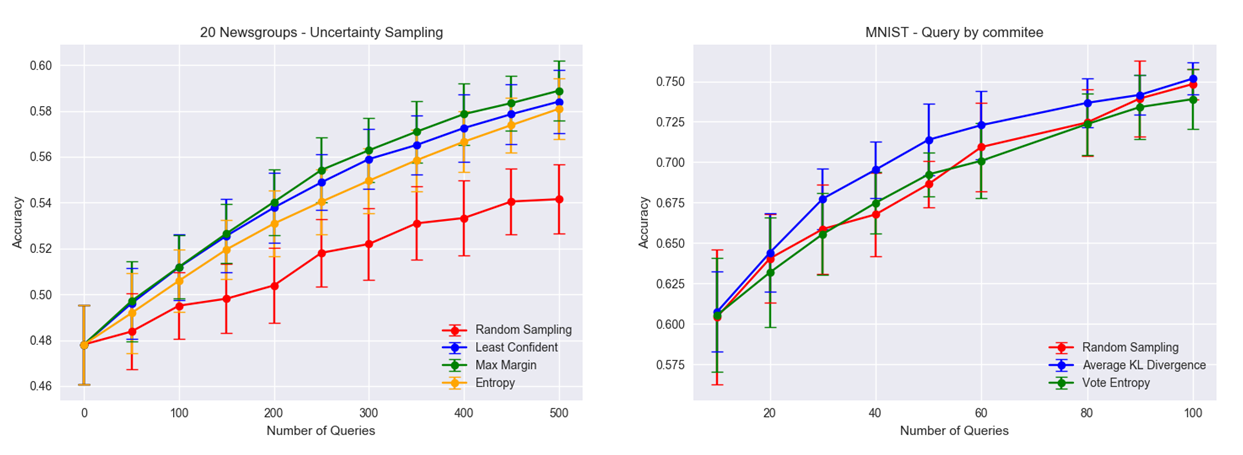
\includegraphics[width=0.95\textwidth, trim={10 10 10 10}]{figures/active_learning_merged.png}
    \caption{Active Learning: Uncertainty Sampling and Query By Committee.}
    \label{fig:al_merged}
\end{figure}

Figure \ref{fig:al_merged} compares $3$ uncertainty sampling techniques: least confident, max margin and entropy with a random subsampling baseline on 20 newsgroups dataset classified with Logistic Regression. All three methods achieve higher accuracy in comparison to baseline that highlights the benefit of active learning. On the right, we can see the performance of Query By Committee strategy applied to MNIST dataset. The committee consists of $5$ instances of Logistic Regression. Two methods are compared against the random subsampling baseline: vote entropy and average KL divergence. We can see that average KL divergence achieves highest classification accuracy. All experiments were repeated $10$ times.  


\subsection{Submodular Optimization}

Many observation selection problems satisfy an intuitive \textbf{diminishing returns} property: adding an observation helps more if we made few observations so far, and helps less if we already made a lot of observations. From a sensing perspective, combining two sets of information has less gain than the sum of information gains of the individual sets. This concept is formalized by the property of submodularity.\\

Submodularity is a property of \textit{set functions} $f: 2^{V} \rightarrow \mathbb{R}$ that assign each subset $S \subseteq V$ a value $f(S)$. $F$ is called \textit{submodular} if for all $A, B \subseteq V$ it holds that
\begin{equation}
    F(A) + F(B) \geq F(A \cup B) - F(A \cap B)
\end{equation}
Note that if $F$ is non-negative ($F(A)\geq 0$ for all $A$) submodularity implies subadditivity: $f(A \cup B) \leq f(A) + f(B)$. An alternative definition of submodular functions is the following. A set function is sub-modular iff for all $A \subseteq B \subseteq V$ and $s \in V \setminus B$, it holds that
\begin{equation}
    F(A \cup \{s\}) - F(A) \geq F(B \cup \{s\}) - F(B) 
\end{equation}
We can usually check more easily for monotonicity and submodularity of a function via its incremental definition, where the increment function $f(A|B)$ is defined as $f(A|B) = f(A \cup B) - f(B)$. Thus, for a single element $\{e\} \in V \setminus B$ and $A \subseteq B \subseteq V$, we can define sub-modularity as:
\begin{equation}
    f(e|A) \geq f(e|B)
\end{equation}
An important subclass of submodular functions are those which are \textit{monotone} where enlarging the argument set cannot cause the function to decrease. A function $f: 2^{V}\rightarrow \mathbb{R}$ is monotone if for every $A \subseteq B \subseteq V$, we have $f(A) \leq f(B)$.

Submodularity is closed under the operations of non-negative addition, restriction and conditioning. 
\begin{theorem}
(Submodularity is closed under conic combination). Given submodular functions $f_1,f_2,...,f_n$ and $\alpha_i \geq 0$, their conic combination (non-negative addition) is submodular.
\begin{equation}
    f(A) = \sum_{i=1}^{n} \alpha_i f_i(A)
\end{equation}
\end{theorem}
\textit{Proof}. Since every function $f_i$ is submodular and $\alpha_i \geq 0$, we have for $A \subseteq B$:
\begin{equation}
    f_i(j|A) \geq f_i(j|B) \Rightarrow \sum_{i=1}^{n}\alpha_i f_i(j|A)\geq \sum_{i=1}^{n}\alpha_i f_i(j|B) \Rightarrow f(j|A) \geq f(j|B)
\end{equation}

\begin{theorem}
(Entropy is submodular). Let $V$ be the index set of a set of random variables, then the following function is submodular:
\begin{equation}
    f(A) = H(X_A) = - \sum_{X_A} p(X_A)\log p(X_A)
\end{equation}
\end{theorem}
\textit{Proof}. For $A \subseteq B \subseteq V$ and $e \in V \setminus B$, we have:
\begin{eqnarray}
    F(A\cup {e}) - F(A) &=& H(X_A,X_e) - H(X_A) = H(X_e|X_A) \\
                        &\geq& H(X_e|X_A, X_B) = H(X_e|X_B) =  H(X_B,X_e) - H(X_B) \\
                        &=& F(B\cup {e}) - F(B)
\end{eqnarray}
where the inequality is due to the fact that conditioning reduces entropy. 

\begin{theorem}
(Mutual Information is submodular). MI is a submodular function if observed variables are conditionally independent given the latent state. 
\end{theorem}
\textit{Proof}. MI can be expressed as a set function $f(A) = I(X;Y_A)$. We make a distinction between latent variables $X$ and observed variables $Y$. For any pair $I, J \subseteq V$ such that $I \cap J = \emptyset$, we assume $Y_I$ is independent of $Y_J$ given $X$. Let $A\subseteq B\subseteq V$, and $j \in V\setminus B$, we have:
\begin{eqnarray}
    I(Y_j; Y_{B\setminus A} | Y_A) &\geq& 0 \\
    H(Y_j|Y_A) - H(Y_j|Y_{(B\setminus A)\cup A}) &\geq& 0 \\
    H(Y_j|Y_A) &\geq& H(Y_j|Y_B)
\end{eqnarray}
which is the submodularity for entropy. Continuing by using conditional independence assumption and subtracting $H(Y_j|X)=H(Y_j|X,Y_A)=H(Y_j|X,Y_B)$ from both sides:
\begin{eqnarray}
    H(Y_j|Y_A) - H(Y_j|X) &\geq& H(Y_j|Y_B) - H(Y_j|X)\\
    H(Y_j|Y_A) - H(Y_j|X,Y_A) &\geq& H(Y_j|Y_B) - H(Y_j|X, Y_B)\\
    I(Y_j;X|Y_A) &\geq& I(Y_j;X|Y_B) \\
    I(X;Y_j|Y_A) &\geq& I(X;Y_j|Y_B) 
\end{eqnarray}

\subsubsection{Greedy Maximization}

Submodular functions arise in many applications and therefore it is natural to study submodular optimization. In particular, we focus on greedy maximization of submodular functions. We are interested in solving problems of the form:
\begin{equation}
    \max_{S\subseteq V} f(S)
\end{equation}
subject to some constraints on $S$. We will focus on two kinds of constraints: \textit{cardinality constraint} $|S| \leq k$ and the \textit{budget constraint} $\mathrm{cost}(S)\leq B$. An example of the former is a sensor placement problem where we want to find the $k$ best sensor locations. An example of the latter is a knapsack problem where we would like to maximize the value of items given a total budget of their weight.\\

A simple greedy approach to maximizing submodular functions is a greedy selection summarized in Algorithm \ref{alg:submodular_1} that starts with an empty set $S_0$ and at iteration $i$, adds the element maximizing the increment function:
\begin{equation}
    S_i = S_{i-1} \cup \{\arg \max_e f(e|S_{i-1})\}
\end{equation}

\begin{algorithm}
\caption{Greedy Algorithm for Maximizing a Submodular Function}
\label{alg:submodular_1}
\begin{algorithmic}[1]
\STATE Init $A_0 = \emptyset$, $k$
\STATE \textbf{for} $j=1,2,...,k$ \textbf{do}
\STATE ~~~ $a_j = \arg \max_{e\in V} f(e|A_{j-1})$ 
\STATE ~~~ set $A_j = A_{j-1} \cup \{a_j\}$ 
\STATE ~~~ set $V = V\setminus \{a_j\}$ 
\STATE \textbf{end for}  
\end{algorithmic}
\end{algorithm}

A celebrated result by Nemhauser \cite{Nemhauser78} proves that that the greedy algorithm provides a good approximation to the optimal solution of the NP-hard optimization problem. 
\begin{theorem}
Let $f : 2^{V} \rightarrow \mathbb{R}$ be a non-negative, monotone submodular function and let $\{S_i\}_{i \geq 0}$ be the greedily selected sets. Then for all positive integers $k$ and $l$:
\begin{equation}
    f(S_l) \geq \bigg(1 - e^{-l/k} \bigg) \max_{S:|S|\leq k} f(S)
\end{equation}
\end{theorem}
\textit{Proof}. Let $S^{\ast} = \arg \max \{f(S): |S| \leq k \}$ be an optimal set of size $k$. Order the elements of $S^{\ast}$ arbitrarily as $\{v_{1}^{\ast},...,v_{k}^{\ast}\}$. Then, we have the following sequence of inequalities for all $i < l$:
\begin{eqnarray}
    f(S^{\ast}) &\leq& f(S^{\ast}\cup S_i) \\
                &=& f(S_i) + \sum_{j=1}^{k} f(v_{j}^{\ast}| S_i \cup \{v_{1}^{\ast},...,v_{j-1}^{\ast}\}) \\
                &\leq& f(S_i) + \sum_{v\in S^{\ast}} f(v|S_i)\\
                &\leq& f(S_i) + \sum_{v\in S^{\ast}} (f(S_{i+1})-f(S_i)) \\
                &\leq& f(S_i) + k(f(S_{i+1})-f(S_i))
\end{eqnarray}
where the first inequality follows from monotonicity of $f$, the second equality is a telescoping sum, the third inequality is follows from the submodularity of $f$, the fourth holds because $S_{i+1}$ is built greedily from $S_i$, and the last inequality reflects the fact that $|S^{\ast}| \leq k$. Therefore,
\begin{equation}
    f(S^{\ast}) - f(S_i) \leq k(f(S_{i+1})-f(S_i))
\end{equation}
Define $\delta_i = f(S^{\ast}) - f(S_i)$, we can then re-write the above expression as $\delta_i \leq k (\delta_i - \delta_{i+1})$, that can be re-arranged to yield:
\begin{equation}
    \delta_{i+1} \leq \bigg(1-\frac{1}{k}\bigg) \delta_i
\end{equation}
Therefore, $\delta_l \leq (1-\frac{1}{k})^{l}\delta_0$. Using the inequality $1-x \leq e^{-x}$, we have
\begin{equation}
    \delta_l \leq \bigg(1-\frac{1}{k}\bigg)^{l}\delta_0 \leq e^{-l/k}f(S^{\ast})
\end{equation}
where we used the fact that $\delta_0 = f(S^{\ast}) - f(\emptyset) \leq f(S^{\ast})$ since $f$ is non-negative by assumption. Substituting $\delta_l = f(S^{\ast}) - f(S_l)$ and re-arranging, we get:
\begin{equation}
    f(S_l) \geq (1-e^{-l/k})f(S^{\ast})
\end{equation}
Therefore, if we let the greedy algorithm pick $l=k$ sensors (compared to the optimal set of size $k$), the greedy solution is no worse than $1-1/e \approx 0.632$ of the optimal value!\\

\begin{figure}[tbhp]
    \centering
    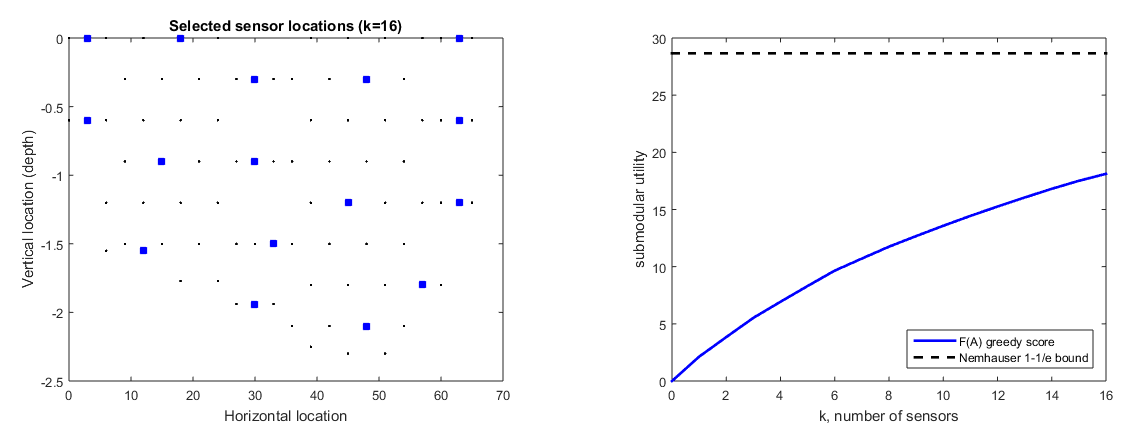
\includegraphics[width=0.95\textwidth, trim={10 10 10 10}]{figures/sfo_sensors_merged.png}
    \caption{Submodular function optimization subject to cardinality constraint.}
    \label{fig:sensors_merged}
\end{figure}

Figure \ref{fig:sensors_merged} shows a sensor selection problem that maximizes mutual information $F_{mi}(A) = H(V\setminus A) - H(V\setminus A | A)$ over the ground set $V$ subject to cardinality constraint: $|S| \leq k$. We can see that the selected sensors evenly cover the geographic area. Also shown are submodular utility scores along with Nemhouser bound obtained by taking the last score and dividing it by $(1-1/e)$.    

In many applications, the elements $v \in V$ may have non-uniform costs $c(v)\geq 0$ and we may want to maximize $f$ subject to a budget $B$ that the total cost cannot exceed:
\begin{equation}
    \max_S f(S) s.t. \sum_{v \in S} c(v) \leq B
\end{equation}
The standard (uniform cost) greedy algorithm can perform arbitrarily badly since it ignores the cost. Therefore, we need to modify the selection step by normalizing the increment function by the element's cost:
\begin{equation}
    S_{i+1} = S_i \cup \bigg\{ \arg \max_{v \in V\setminus S_i : c(v)\leq B-c(S_i)} \frac{f(v|S_i)}{c(v)} \bigg\}
\end{equation}
Thus, we choose an element that has highest incremental gain and lowest cost. Note that the sensor selection problem can be thought of as a special case of the budget constrained problem if we assign unit costs to all measurements and set the budget $B=k$. Let $S_{uc}$ be the uniform cost solution and $S_{cb}$ be the cost-benefit greedy solution described above. It can be shown that:
\begin{equation}
    \max\{f(S_{uc}),f(S_{cb})\} \geq \frac{1-1/e}{2}\mathrm{OPT} 
\end{equation}

The submodular maximization algorithm with a budget constraint also known as Cost-Effective Lazy Forward-selection (CELF) Algorithm is summarized in Algorithm \ref{alg:celf}.

\begin{algorithm}
\caption{Cost-Effective Lazy Forward-selection (CELF)}
\label{alg:celf}
\begin{algorithmic}[1]
\STATE Input: Reward function $F$, cost function $C$, budget $B$
\STATE ~~~ $A_{UC} = \mathrm{LazyForward}(F,C,B,'UC')$
\STATE ~~~ $A_{CB} = \mathrm{LazyForward}(F,C,B,'CB')$
\STATE ~~~ return $\arg \max \{F(A_{UC}),F(A_{CB})\}$
\STATE LazyForward(F,C,B,type)
\STATE ~~~ 
\STATE \textbf{end for}  
\end{algorithmic}
\end{algorithm}



\begin{figure}[tbhp]
    \centering
    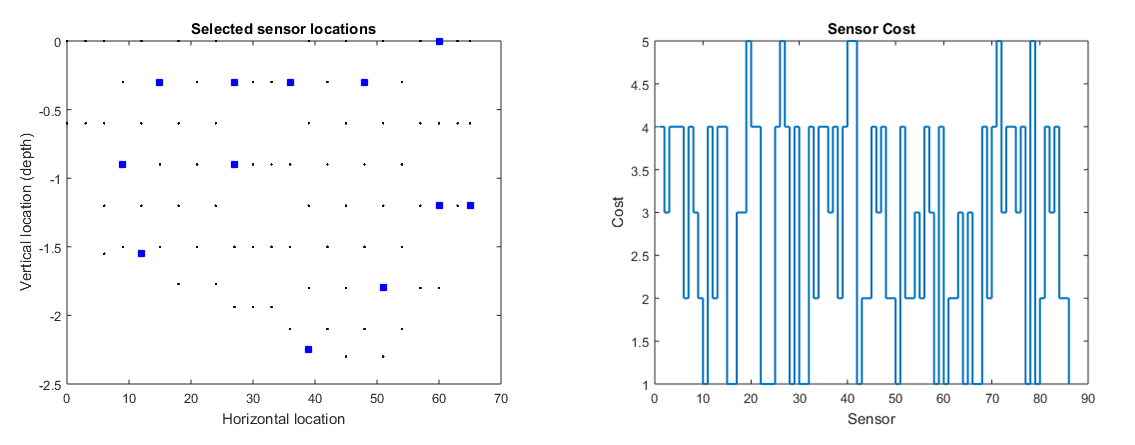
\includegraphics[width=0.95\textwidth, trim={10 10 10 10}]{figures/sfo_budget_merged.png}
    \caption{Submodular function optimization subject to budget constraint.}
    \label{fig:sensors_budget}
\end{figure}







